%TEX root = ../dissertation.tex

\chapter{Pulsarcast}
\label{chapter:pulsarcast}

In this chapter we will introduce and describe our solution. Pulsarcast is a
peer to peer, pub-sub, topic based system focused on reliability, eventual
delivery guarantees and data persistence. We seek this while not fully
compromising the scalability given by the decentralised nature of our
architecture. Looking through our related work it became clear that few fully
decentralised solutions exist that try provide these kind of guarantees. Yet,
if we carefully look at the most popular and widely adopted centralised pub-sub
solutions it is clear that most of them heavily rely and depend upon these same
guarantees. 

We opted for the simpler topic based subscription model given that, in our view, a well structured and implemented topic based model is more than enough for a great percentage of our use cases. In the end, we compromise a bit of the expressiveness of the system in order to avoid bringing more complexity in, something we believe will pay off.

This chapter is divided as follows, we will start by covering the use case of
our system in section \ref{use-case}, where we will introduce some of our
broader architectural decisions. Next, we will move to section
\ref{data-structures} where we will deep dive into Pulsarcast's data structure
model and how it is distributed across the network. Finally, we will look into
one of the most important parts of our architecture in section
\ref{subscription-management-event-dissemination} where, based on the covered
related work and the taxonomy we defined, we present the algorithms and
mechanisms used for managing the subscriptions and event dissemination.

\begin{itemize}
\item Introduzir as decisões de arquitectura
\item Topic based subscriptions
\item Baseado num overlay estruturado (kadmelia DHT) para peer-discovery e
  storage, por cima do qual depois criamos o nosso "overlay"
\item Suporte para sub tópicos
\item Imutabilidade dos dados (tópicos e dados)
\item Nós guardam informação das msgs que recebem
\end{itemize}

\section{Use Case}\label{use-case}

Pulsarcast is a fully decentralised solution, as it has been previously
introduced. This means that each node plays a key part in fulfilling the system
purpose, delivering events and ensuring its dissemination. From a broader
perspective Pulsarcast relies on two overlays to fulfil its needs. Kadmelia
DHT, used for a range of purposed from peer discovery, content discovery and to
bootstrap our other overlay, the Pulsarcast overlay. The Pulsarcast overlay are
actually a set of different overlays or, as we call it, dissemination trees.
These trees are on a per topic basis and are the key factor in the way we
disseminate information across our decentralised network.
 
\begin{figure}[hb!]
  \centering
  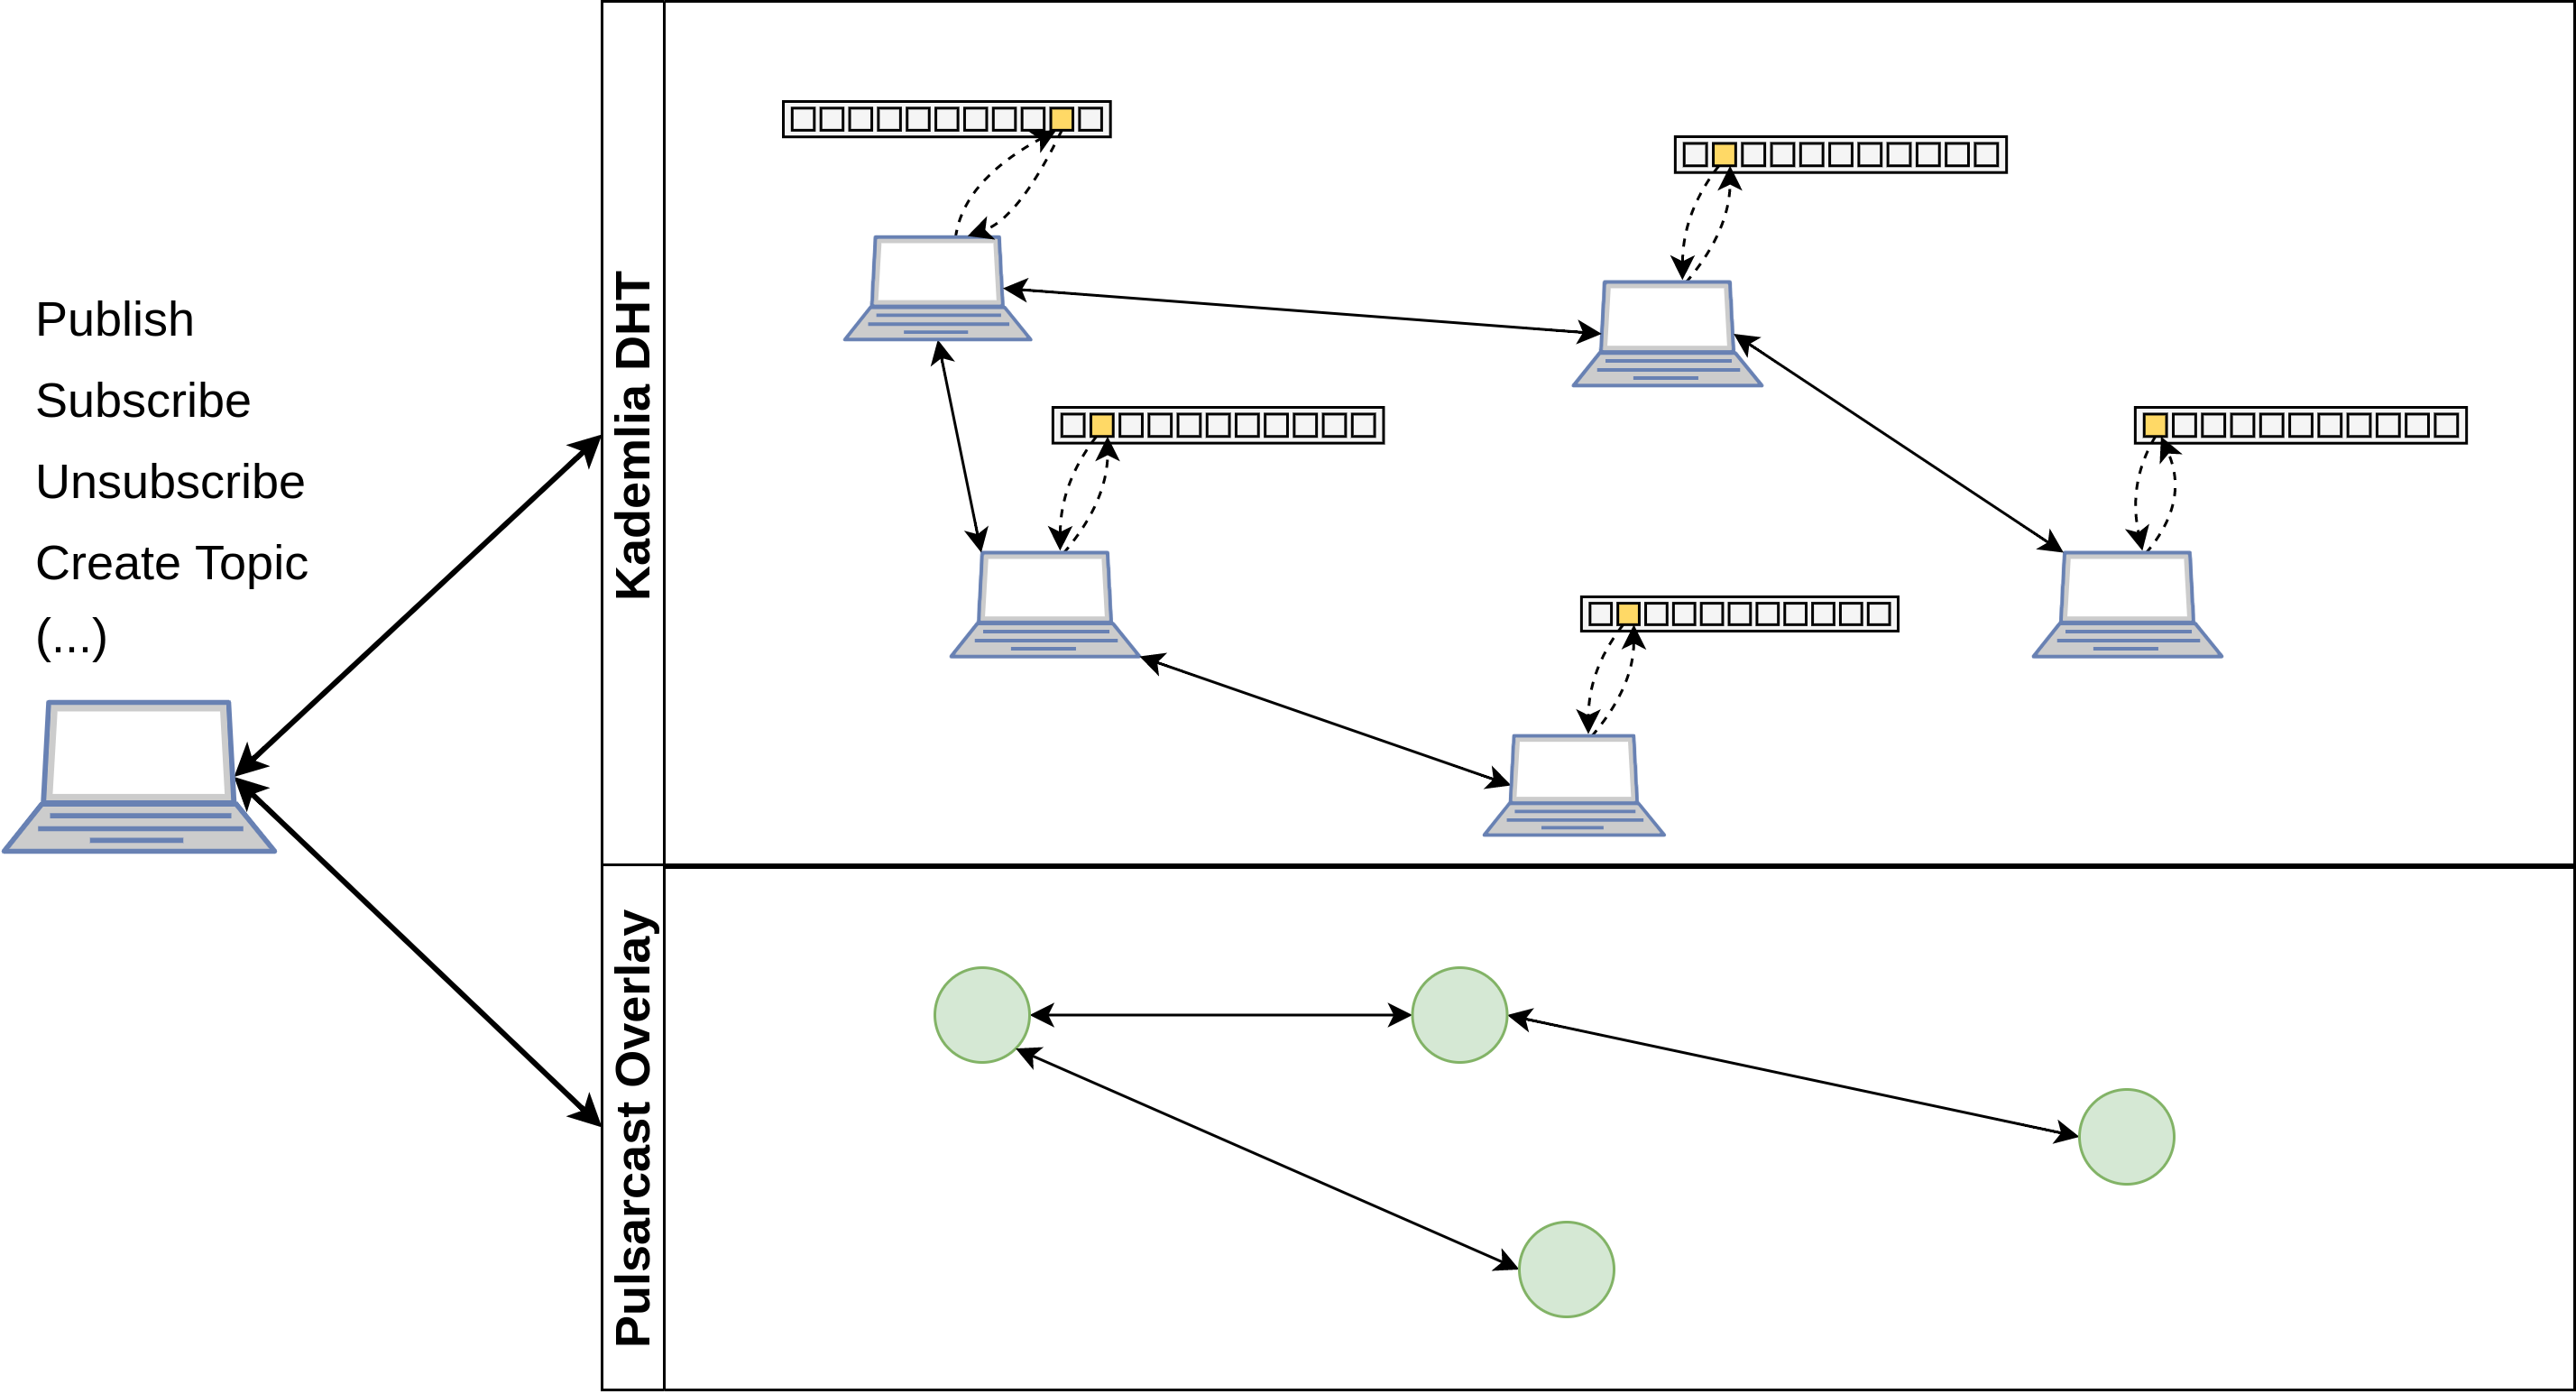
\includegraphics[width=0.95\textwidth]{img/pulsarcast-overlays.png}
  \caption{Representation of the Pulsarcast overlays}
  \label{fig:pulsarcast-overlays}
\end{figure}

When a peer publishes an event TODO


\section{Data Structures}\label{data-structures}

TODO

\begin{itemize}
\item Introduzir conceito de event descriptor e topic descriptor
\item Abordar imutabilidade mais a fundo
\item JSON schemas de Topic Descriptor, Event Descriptor e RPC messages
\item Meta topic
\end{itemize}

TODO

\begin{lstlisting}[language=JSON,caption={Topic descriptor schema in a JSON based format},label={topic-descriptor},captionpos=b]
{
  "name": <string>,
  "author": <peer-id>,
  "parent": {                     //The parent link for this topic
    "/": <topic-id>
  },
  "#": {                          //Sub topic links
    <topic-name>: {
      "/": <topic-id>
    },
    ...
  },
  "metadata": {
    "created": <date-iso-8601>,
    "protocolVersion": <string>,  //Pulsarcast protocol version
    "allowedPublishers": {        //If enabled, whitelist of allowed publishers
      "enabled": <boolean>,
      "peers": [ <peer-id> ]
    },
    "requestToPublish": {         //Enable request to publish
      "enabled": <boolean>,
      "peers": [ <peer-id> ]      //Optional whitelist able to request
    },
    "eventLinking": <string>,     //One of: LAST_SEEN, CUSTOM
  }
}
\end{lstlisting}

TODO

\begin{lstlisting}[language=JSON,caption={Event descriptor schema in a JSON based format},label={event-descriptor},captionpos=b]
{
  "name": <string>,
  "publisher": <peer-id>,         //Peer who published the event
  "author": <peer-id>,            //Author of the event
  "parent": {                     //The parent link for this event
    "/": <topic-id>
  },
  "topic": {
    "/": <topic-id>
  },
  "payload": <binary-data>
  "metadata": {
    "created": <date-iso-8601>,
    "protocolVersion": <string>,  //Pulsarcast protocol version
  }
}
\end{lstlisting}

TODO

\begin{figure}[hb!]
  \centering
  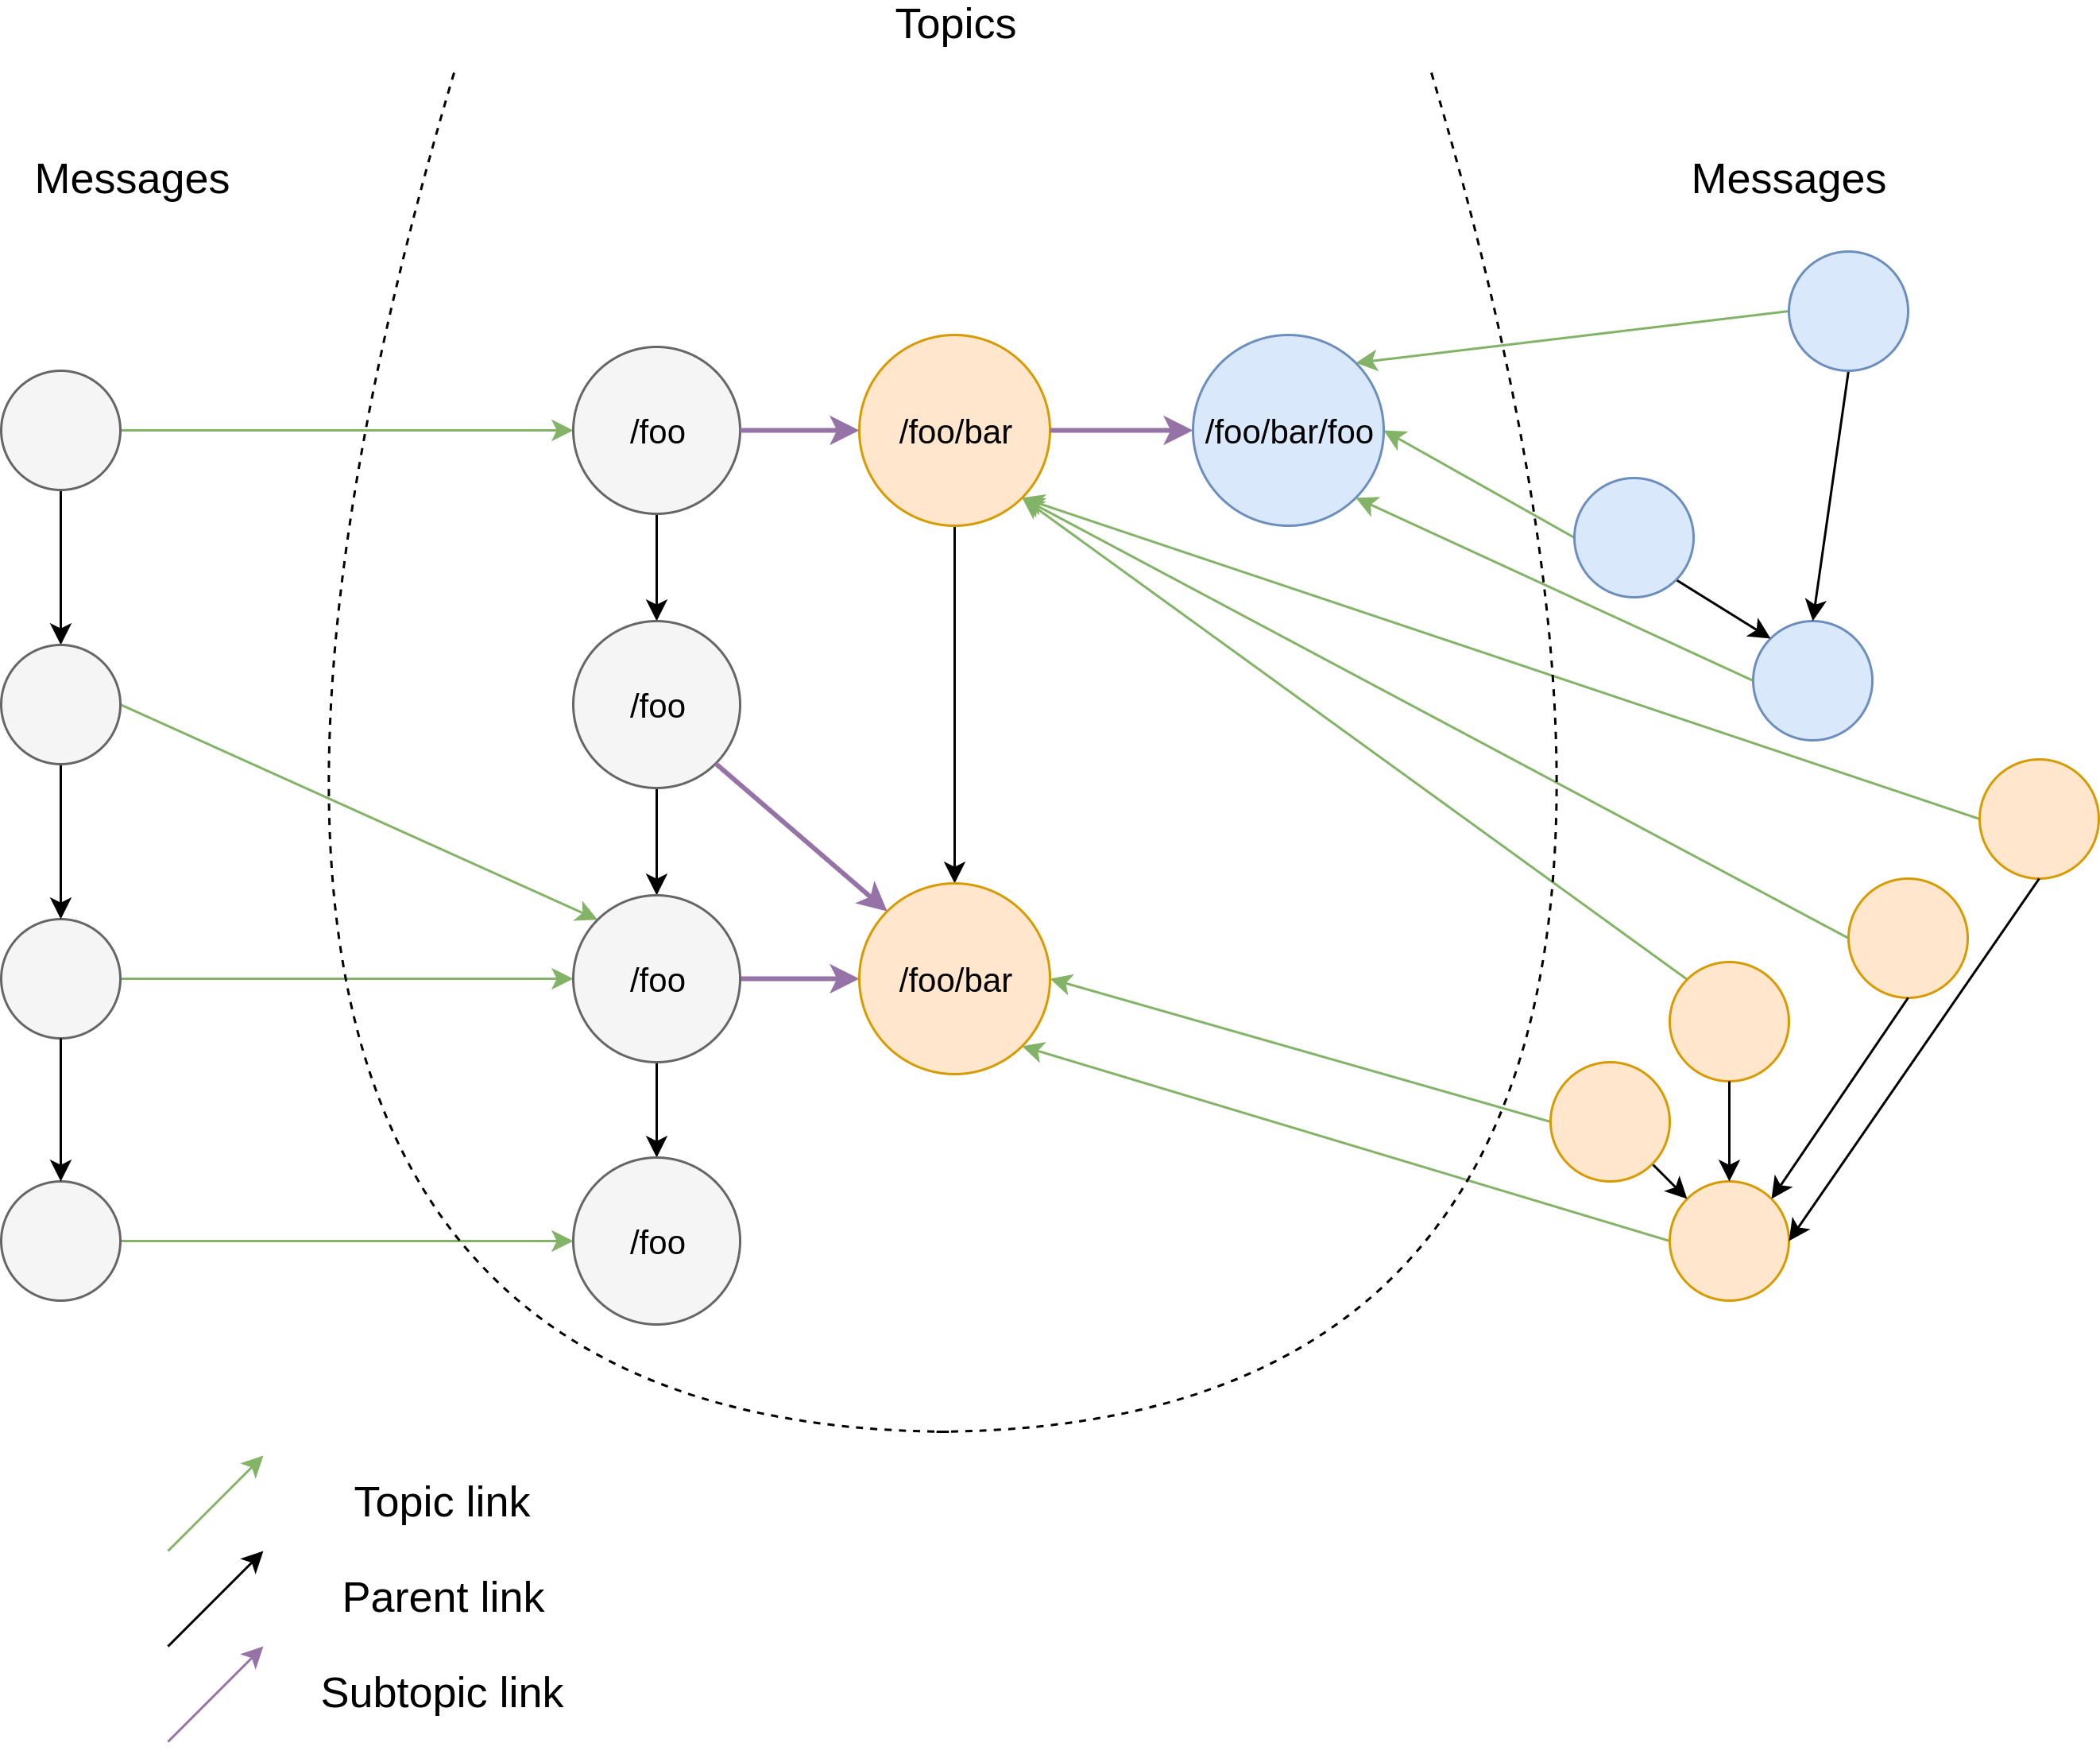
\includegraphics[width=0.95\textwidth]{img/pulsarcast-dag.png}
  \caption{Representation of the Pulsarcast DAG}
  \label{fig:pulsarcast-dag}
\end{figure}

TODO

\begin{figure}[hb!]
  \centering
  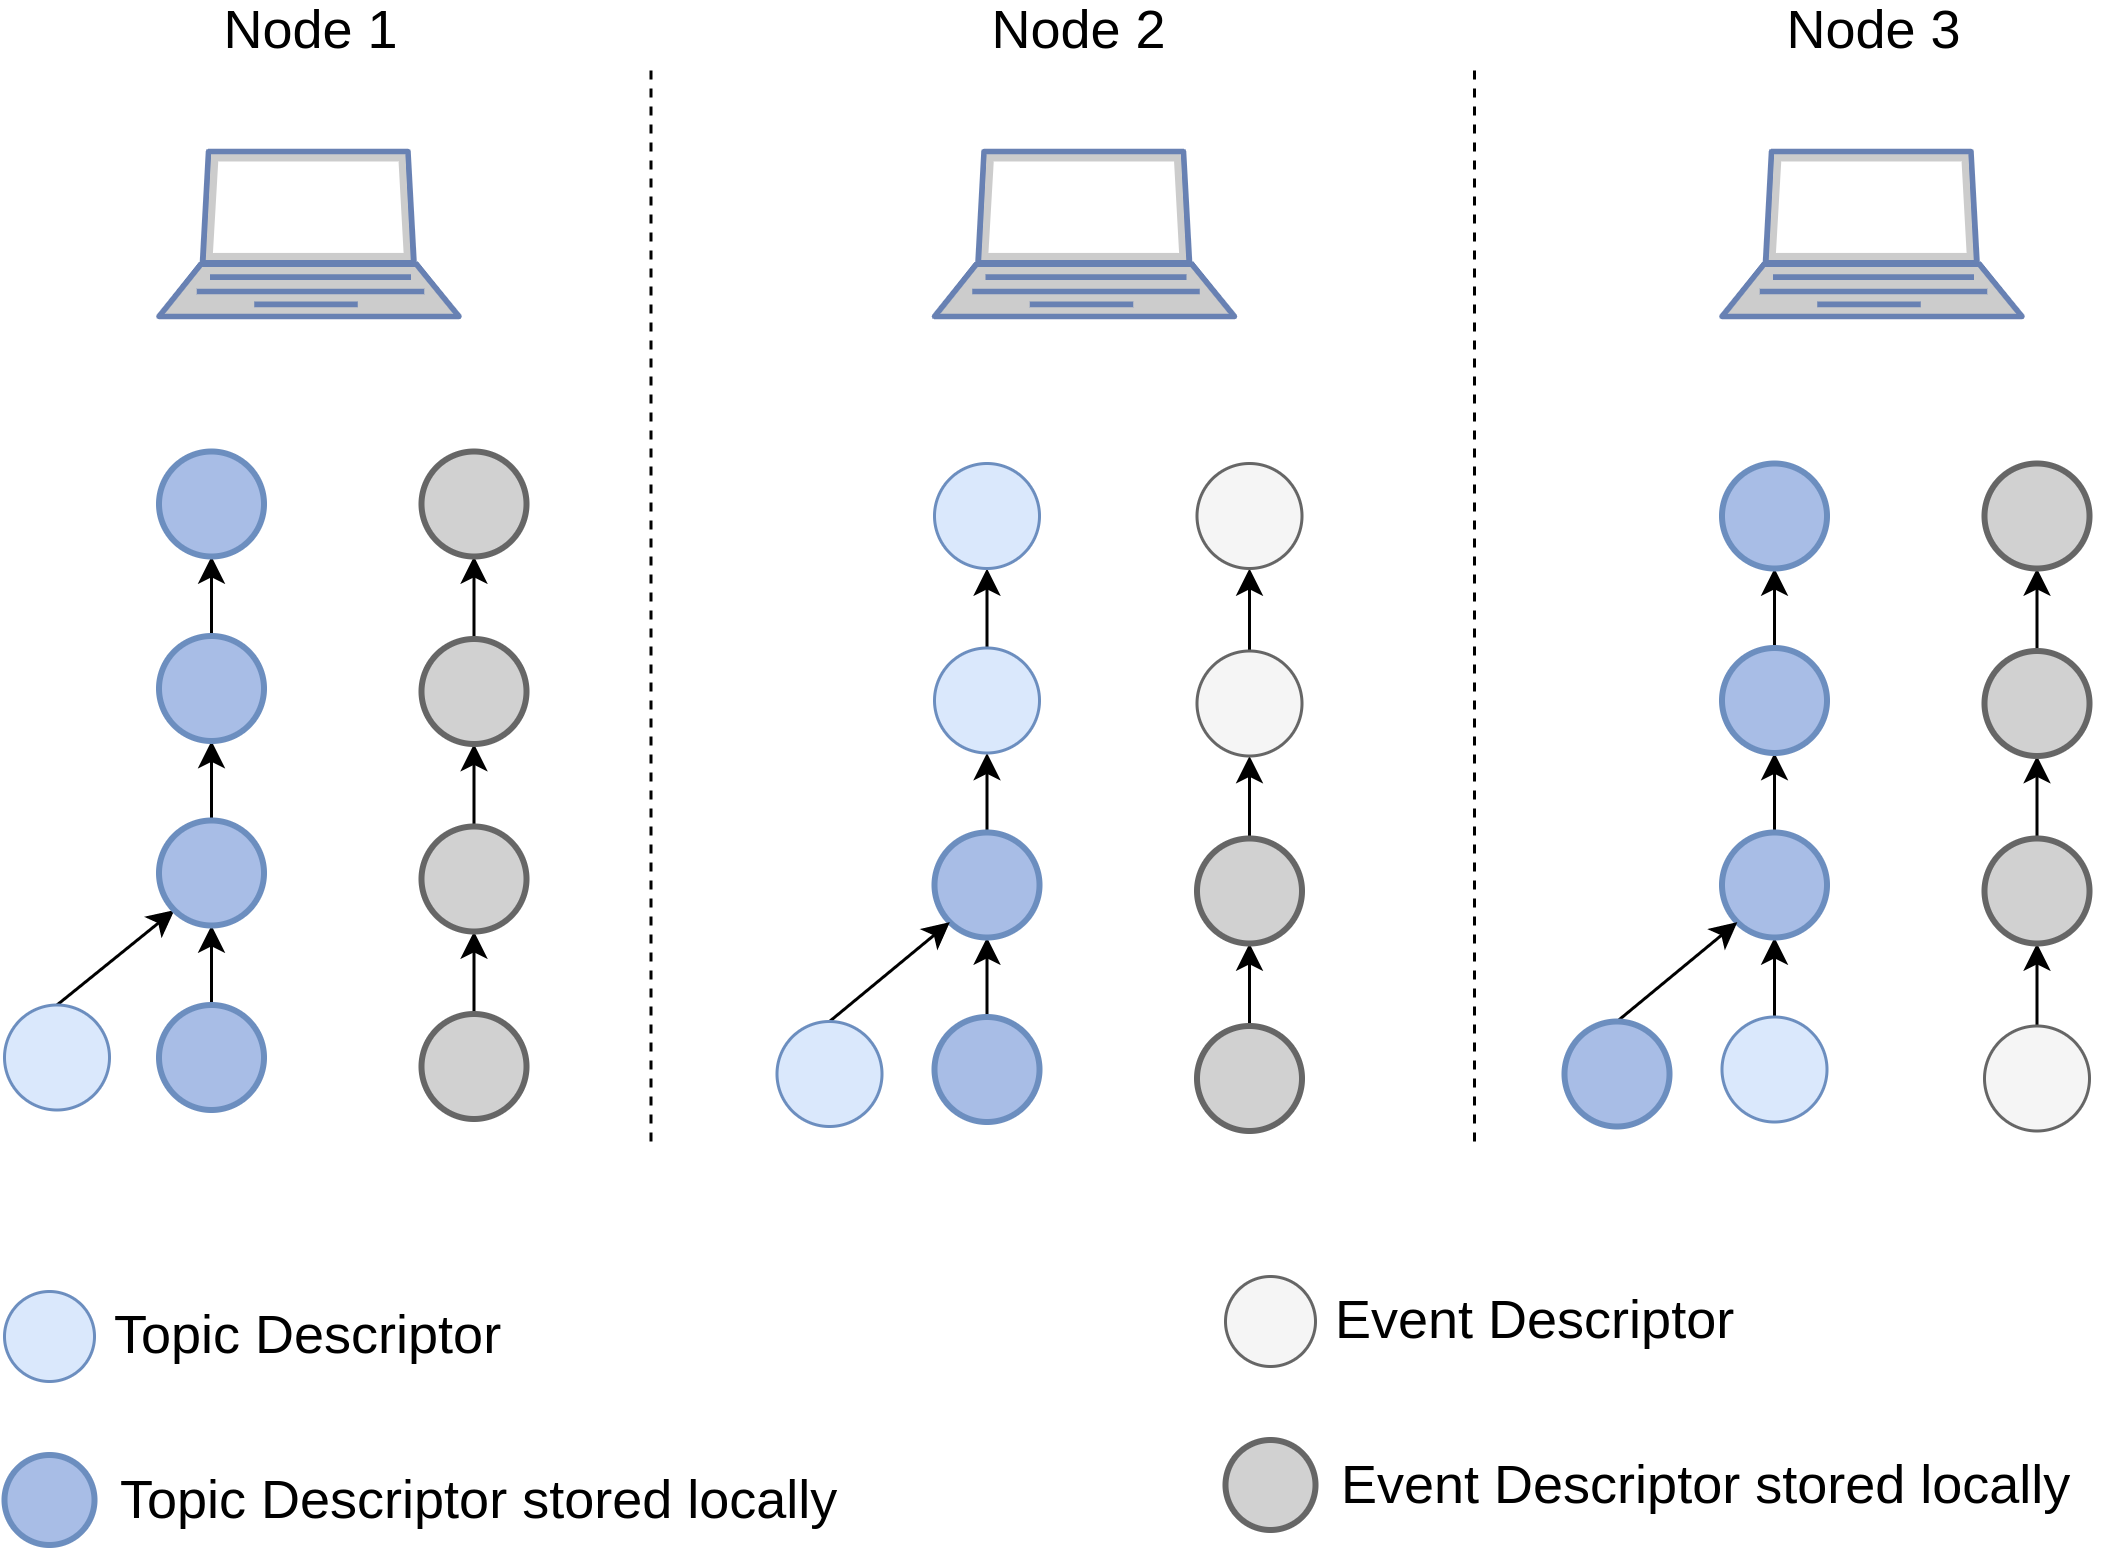
\includegraphics[width=0.95\textwidth]{img/pulsarcast-local-vs-distributed-state.png}
  \caption{Overview of how state is kept across the network}
  \label{fig:pulsarcast-local-vs-distributed-state}
\end{figure}

TODO

\begin{figure}[hb!]
  \centering
  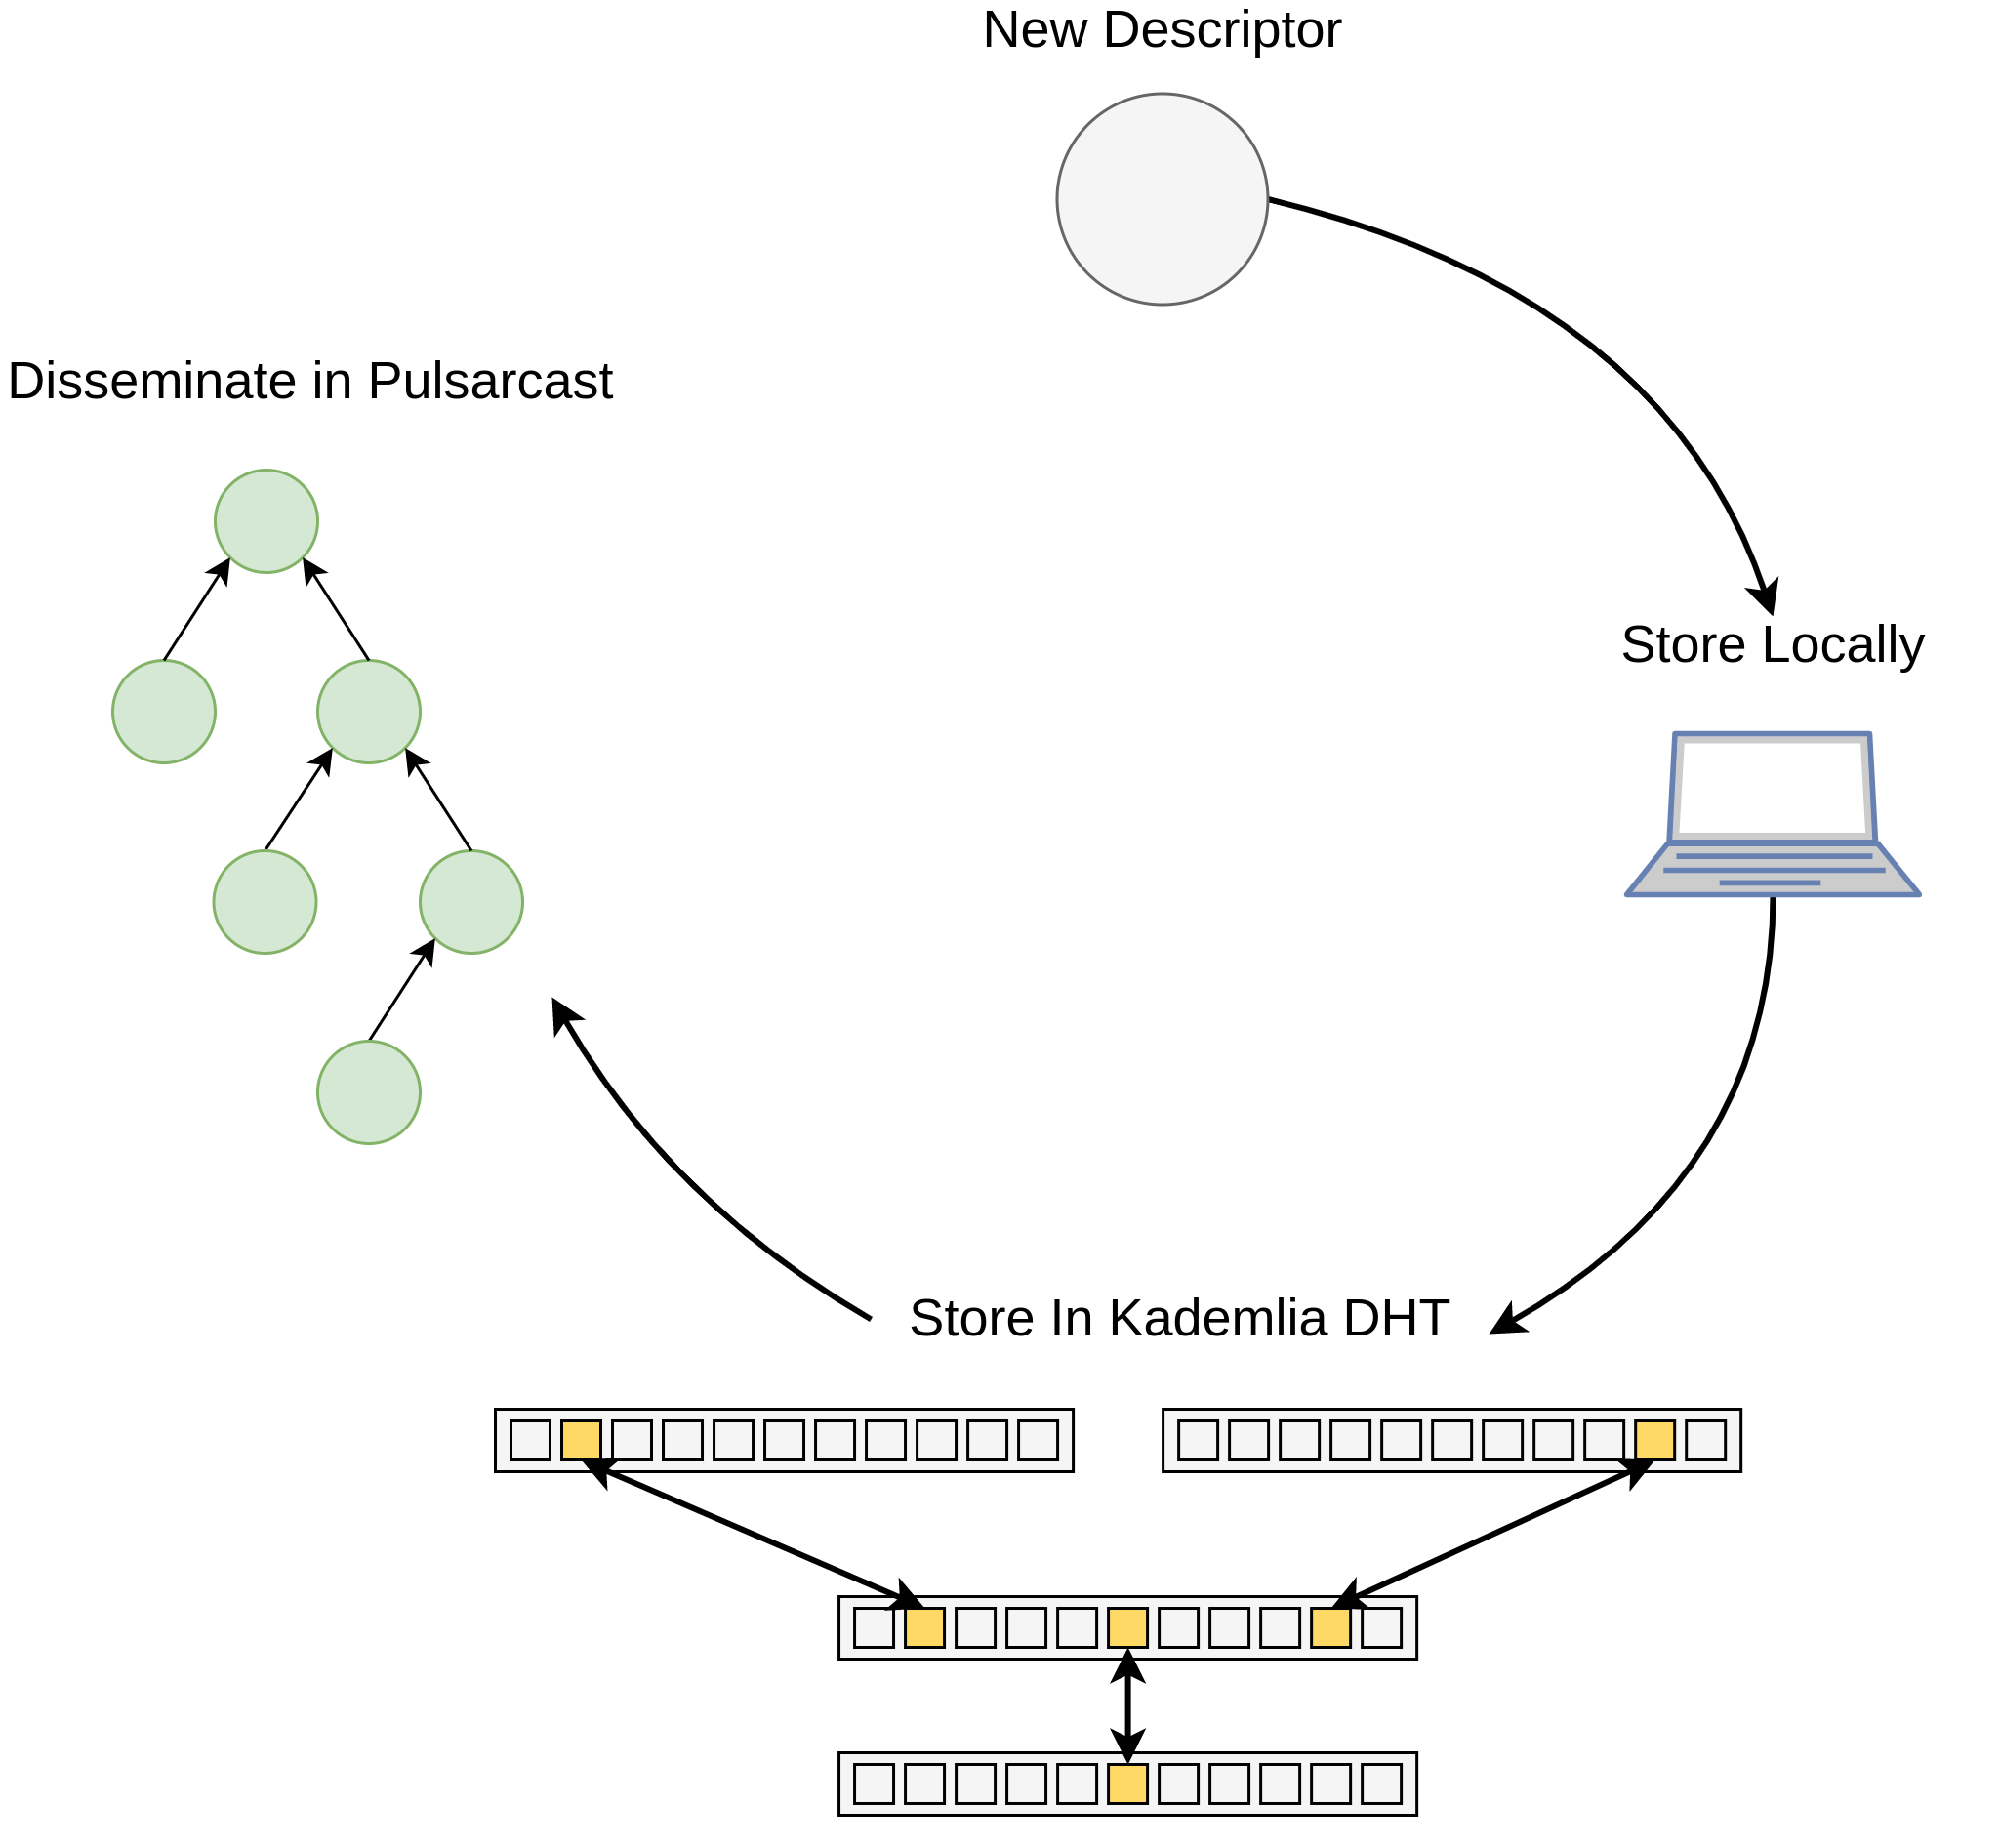
\includegraphics[width=0.95\textwidth]{img/pulsarcast-descriptor-creation.png}
  \caption{Flow for creating a new Topic/Event descriptor}
  \label{fig:pulsarcast-descriptor-creation}
\end{figure}

TODO

\begin{figure}[hb!]
  \centering
  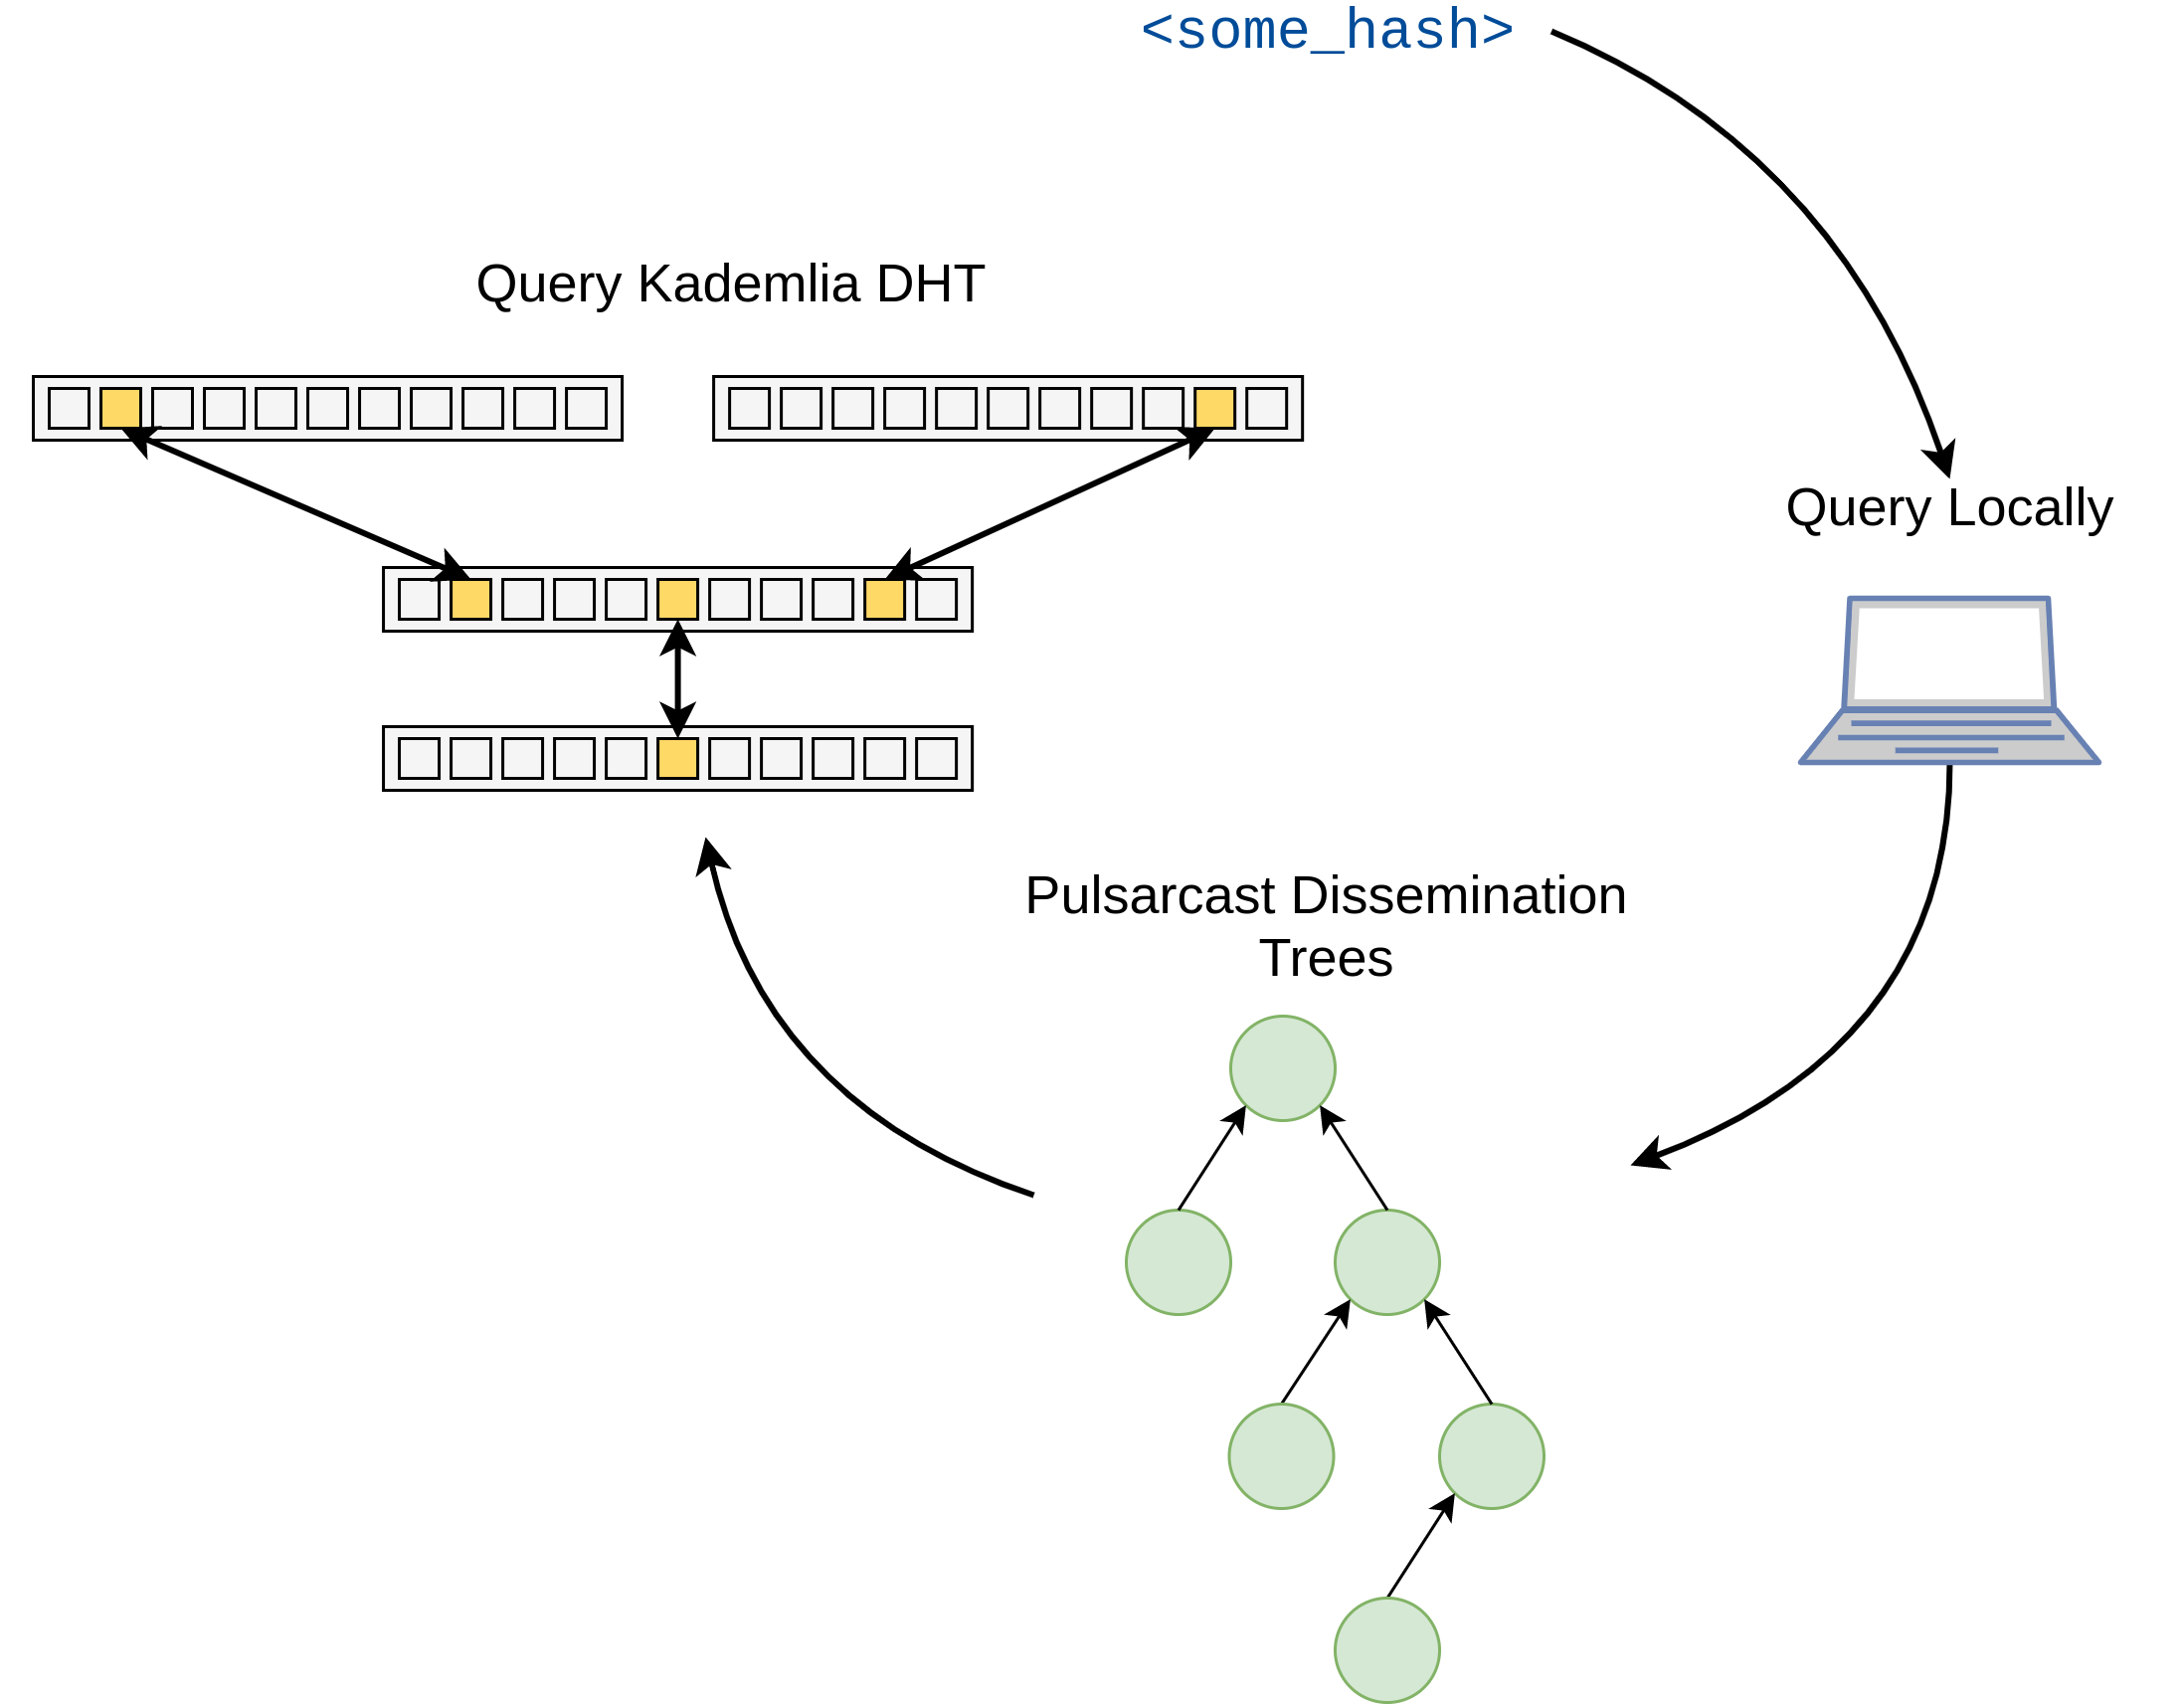
\includegraphics[width=0.95\textwidth]{img/pulsarcast-descriptor-query.png}
  \caption{Flow for querying a Topic/Event descriptor}
  \label{fig:pulsarcast-descriptor-query}
\end{figure}

TODO

\section{Subscription Management and Event Dissemination}\label{subscription-management-event-dissemination}

TODO
\begin{itemize}
\item Árvores de disseminação
\item Event linking (last seen vs custom)
\item Request to publish
\item Allowed publishers
\item Uso da DHT
\item Algoritmos em detalhe
\item Disseminação de eventos
\end{itemize}

TODO

\begin{figure}[hb!]
  \centering
  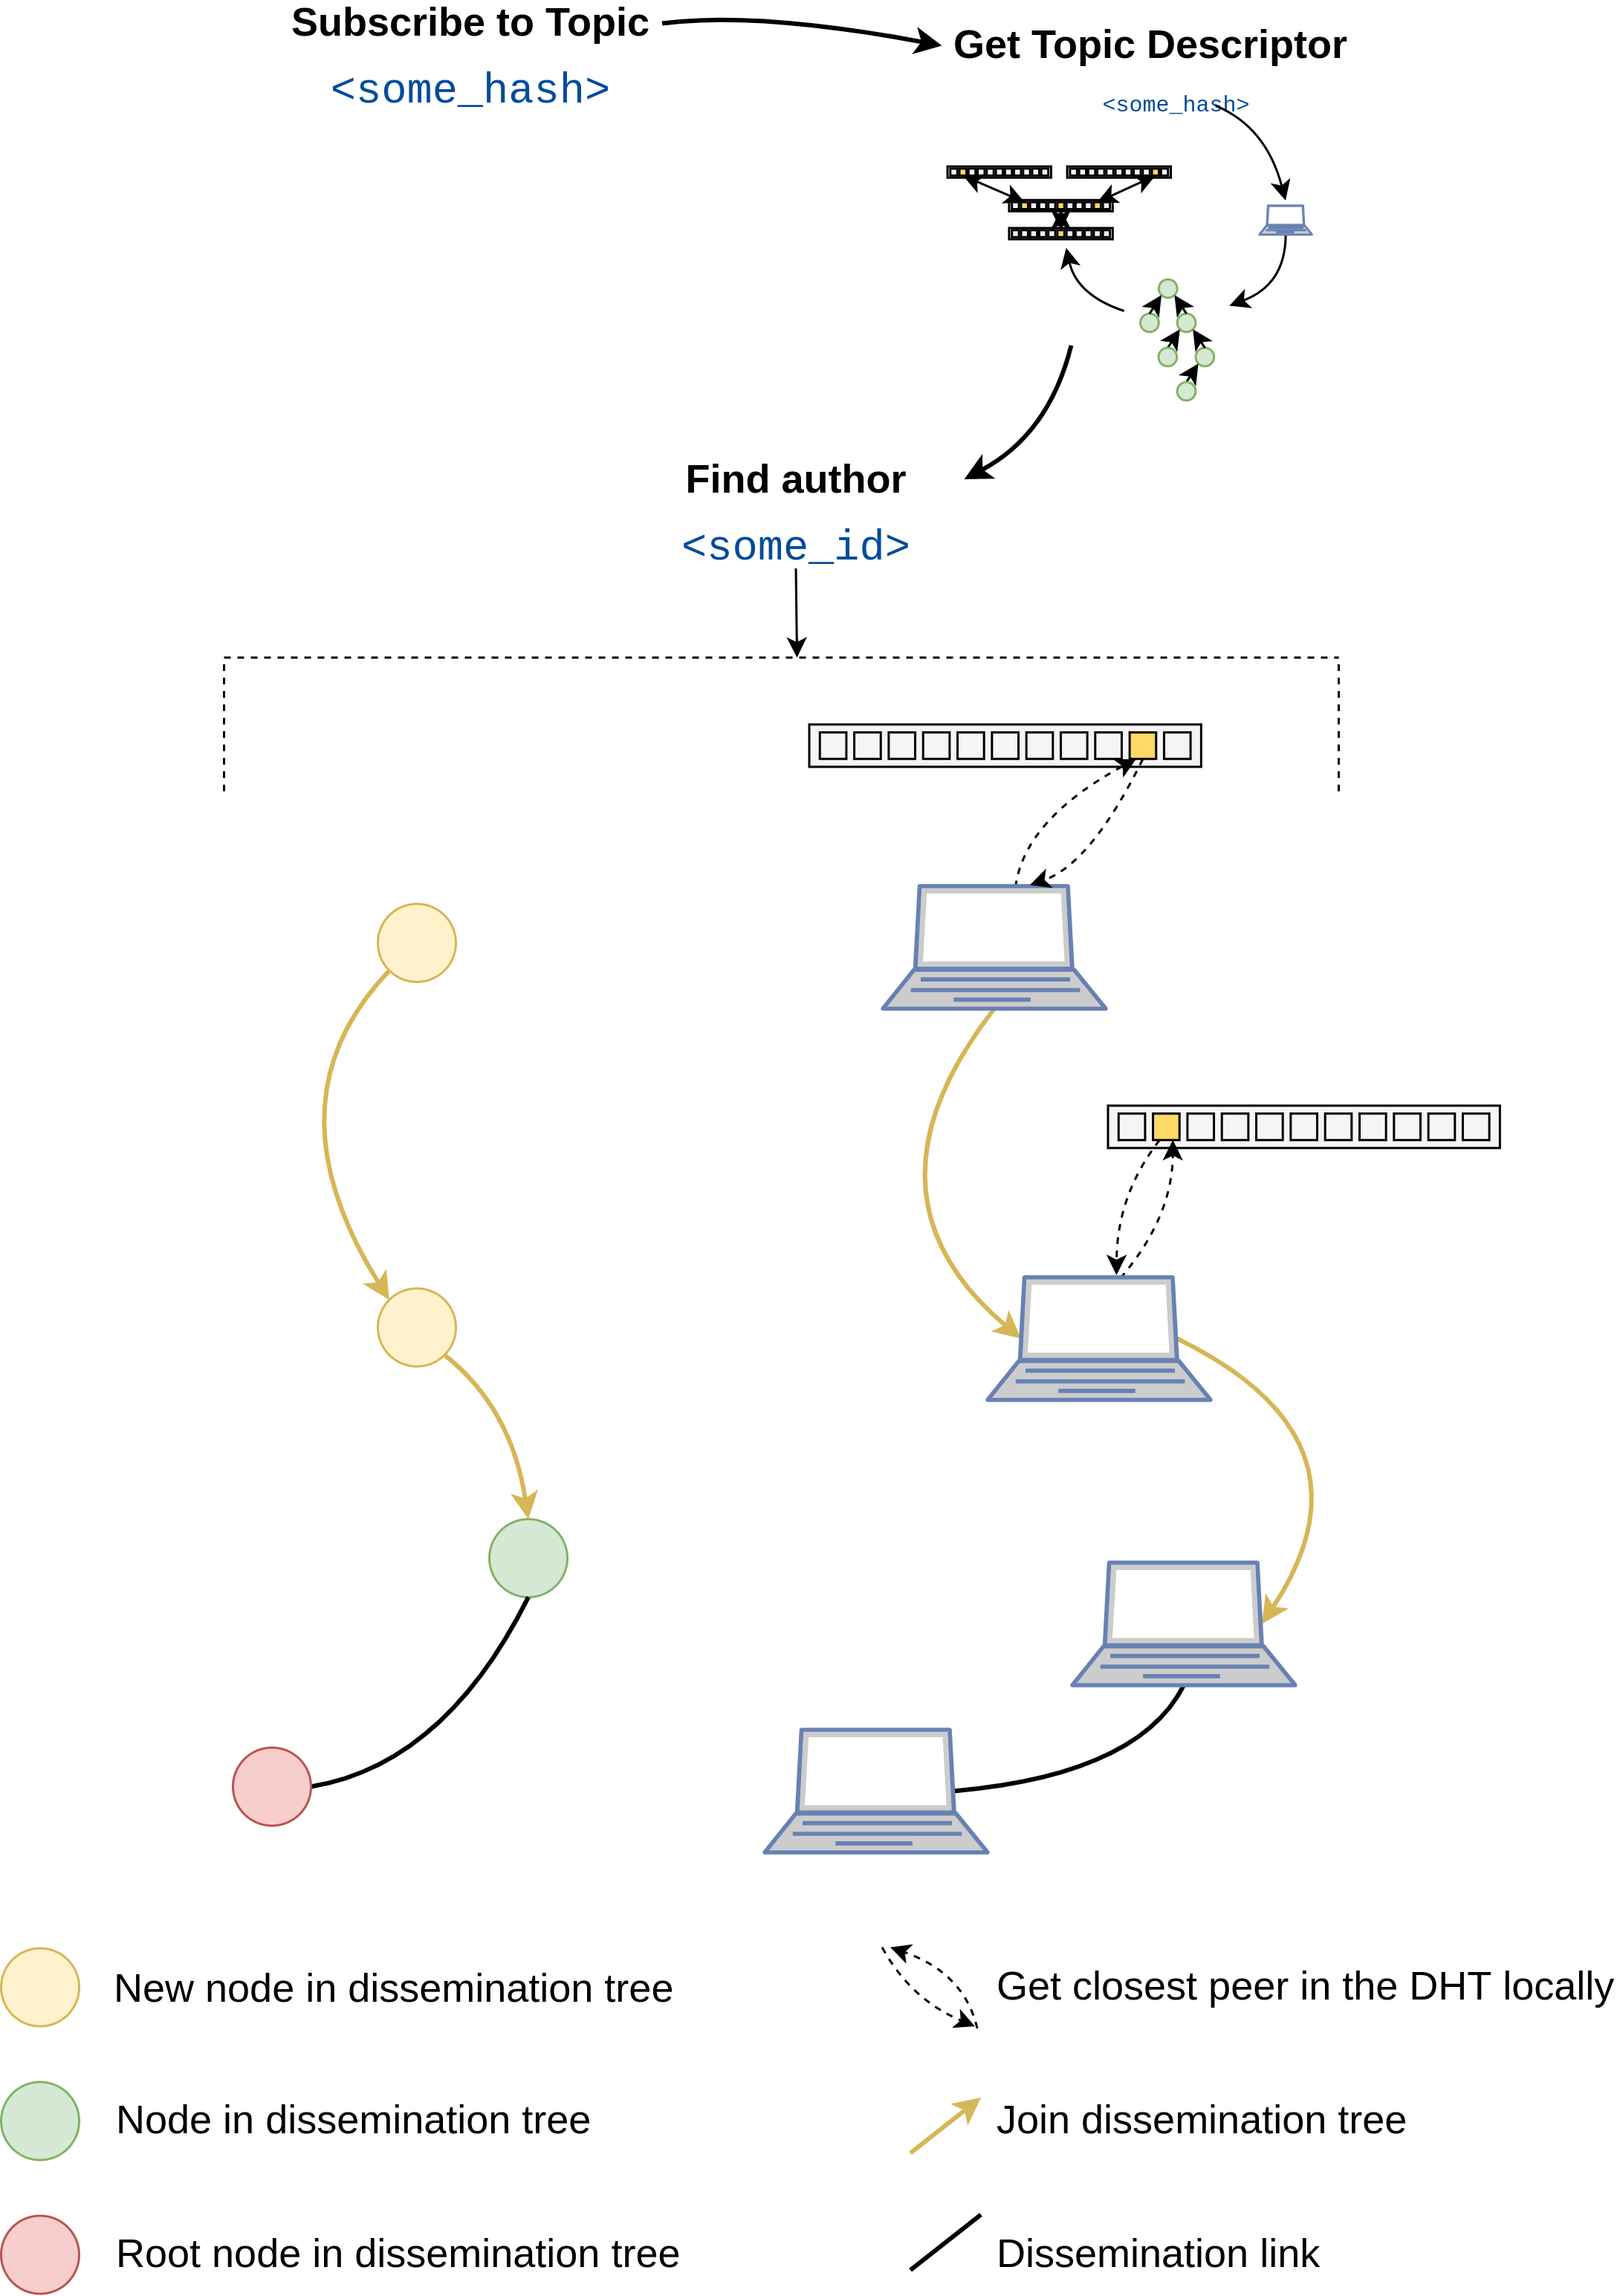
\includegraphics[width=0.95\textwidth]{img/pulsarcast-subscription-flow.png}
  \caption{Overview of the flow for creating a new subscription}
  \label{fig:pulsarcast-subscription-flow}
\end{figure}

TODO

\begin{figure}[hb!]
  \centering
  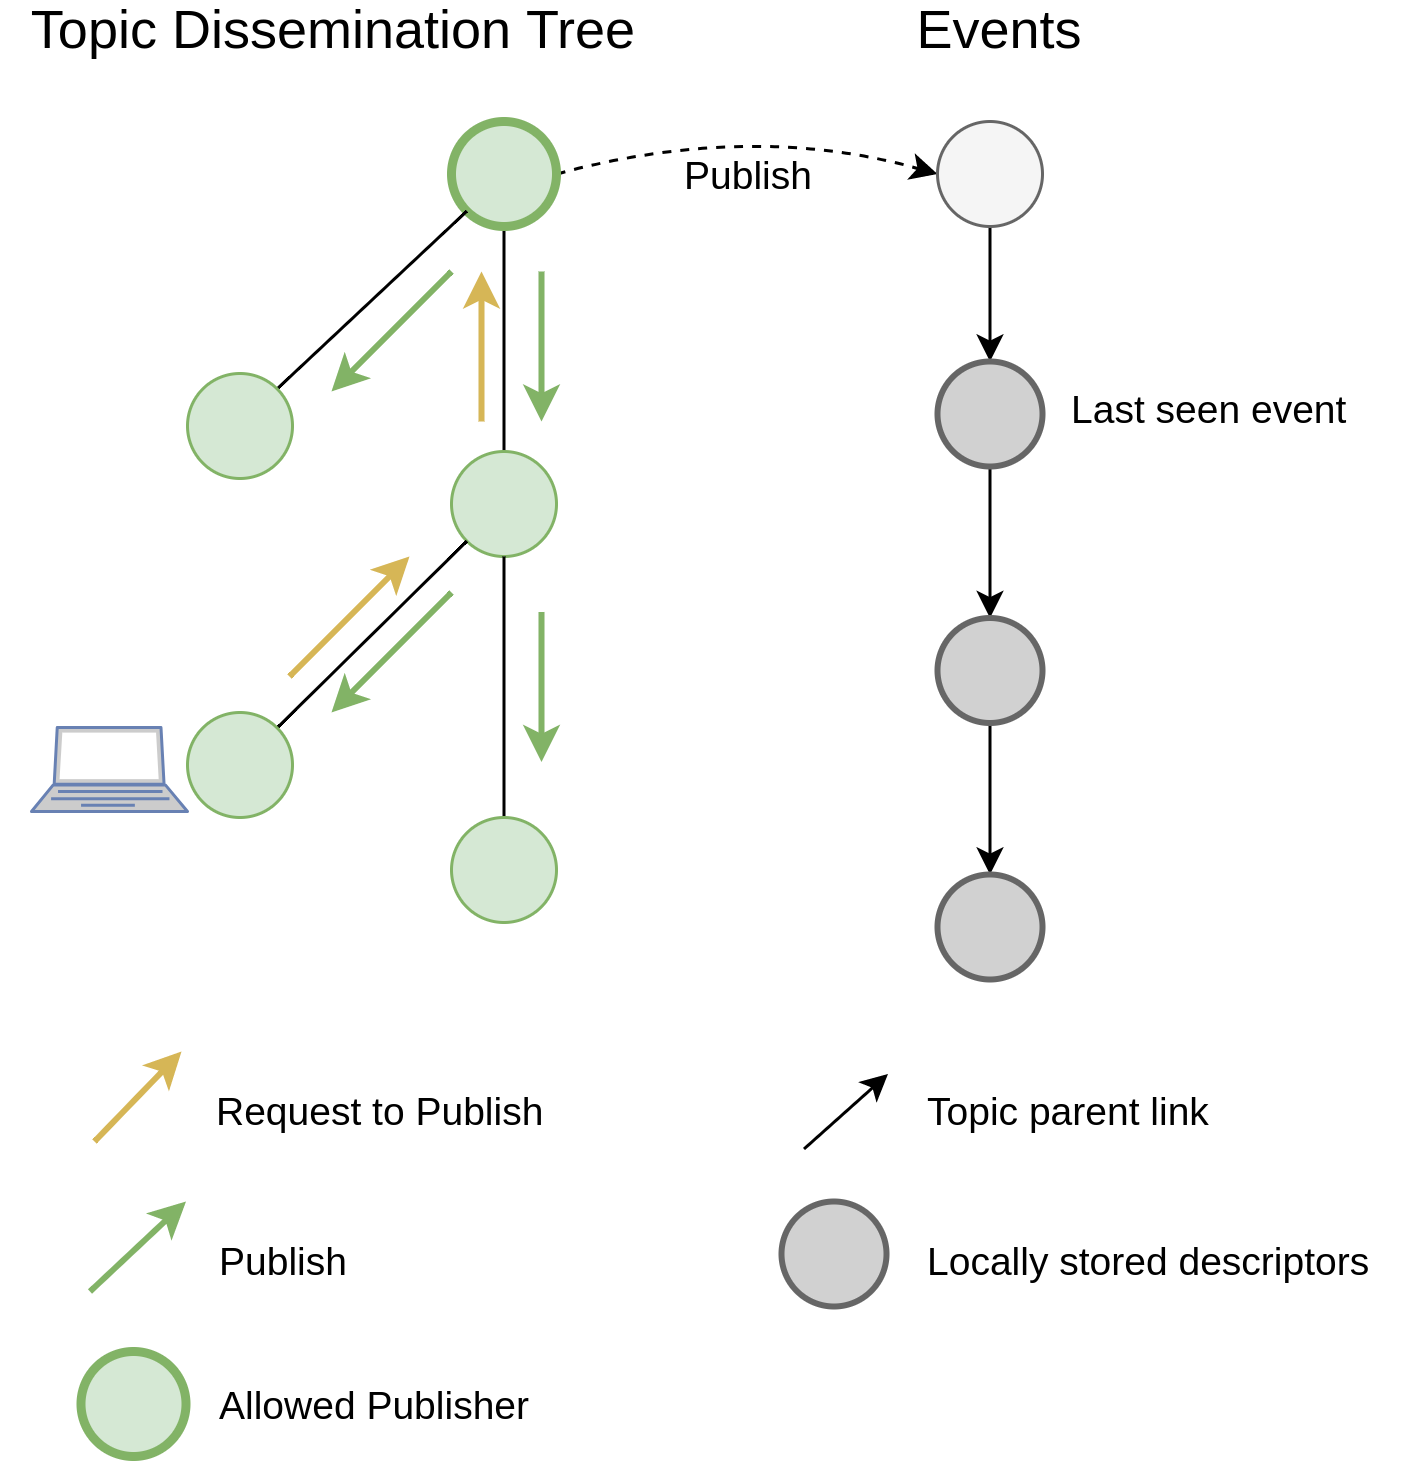
\includegraphics[width=0.95\textwidth]{img/pulsarcast-publish-order-guarantee.png}
  \caption{Event dissemination mechanism for a topic with a order guarantee configuration}
  \label{fig:pulsarcast-publish-order-guarantee}
\end{figure}

TODO

\begin{figure}[hb!]
  \centering
  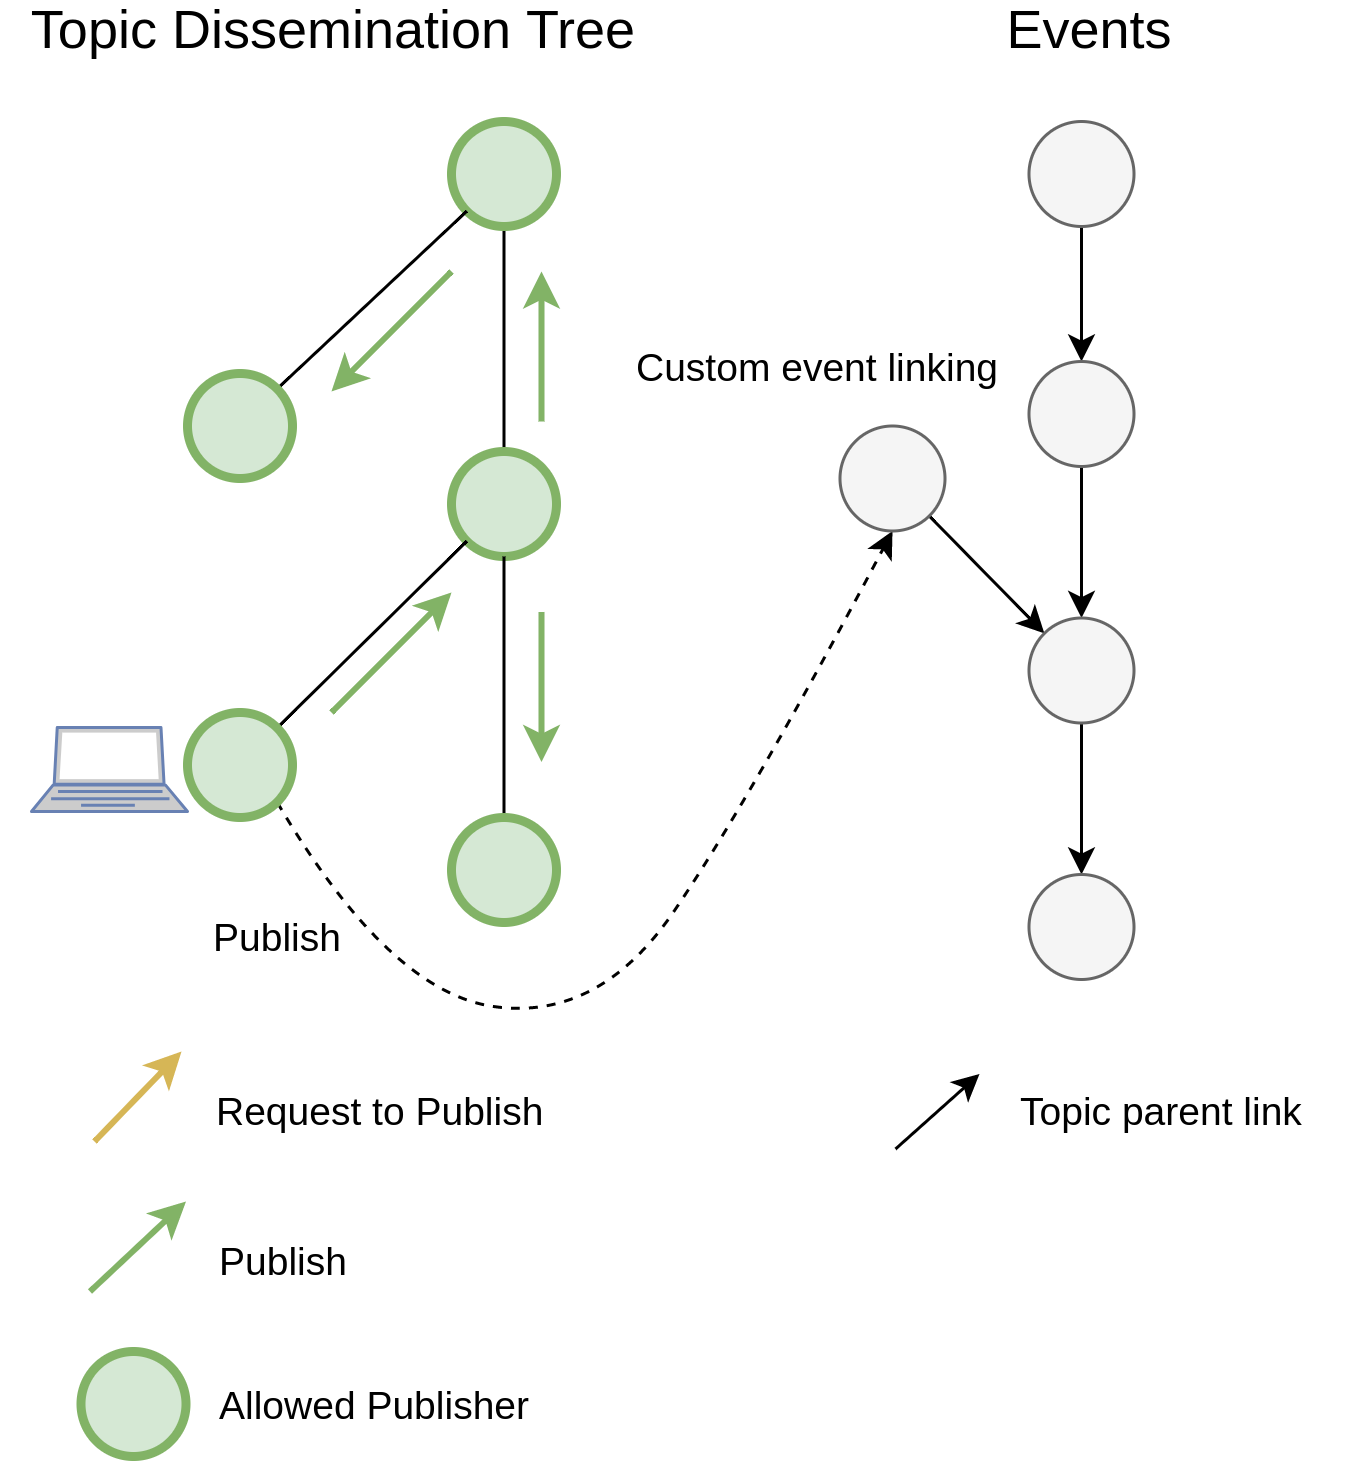
\includegraphics[width=0.95\textwidth]{img/pulsarcast-publish-custom.png}
  \caption{Event dissemination mechanism for a topic with custom event linking and global publishers allowed}
  \label{fig:pulsarcast-publish-custom}
\end{figure}

TODO


\SetKwProg{Fn}{Function}{}{}

\begin{algorithm}[H]
  \SetAlgoLined
  \Fn{CreateTopic(newTopic)}{
  	\KwIn{$newTopic=$ data for new topic creation}
		\BlankLine
  	\Begin{
			$parent \leftarrow newTopic.parent$\;
  	  \eIf(\tcp*[r]{Check if the topic has a parent link}){$parent == null$}{
				$metaTopic \leftarrow CreateMetaTopicDescriptor(newTopic)$\;
  	  }{
				$metaTopic \leftarrow parent.subTopics.meta$\;
			}
			$topicData \leftarrow CreateTopicDescriptor(newTopic, metaTopic)$\;
			$Subscribe(metaTopic)$\;
			$Subscribe(topicData)$\;
			$StoreInDHT(metaTopic)$\;
			$StoreInDHT(topicData)$\;
			$Publish(metaTopic, topicData)$\tcp*[r]{Publish the new topic in the meta topic}\
  	}
	}
  \caption{Create a new topic}
\end{algorithm}

TODO

\begin{algorithm}[H]
  \SetAlgoLined
  \Fn{ReceivedJoin(fromNodeId, topicId)}{
  	\KwData{$nodeId=$ node id of this node}
  	\KwIn{$topicId=$ topic id}
  	\KwIn{$fromNodeId=$ node who we got the join request from}
		\BlankLine
  	\Begin{
  	  $topicData \leftarrow GetTopicData(topicId)$\;
  	  \eIf{$fromNodeId \neq nodeId$}{
        $AddToChildren(t, fromNodeId)$\tcp*[r]{Add as children in dissemination tree}\
				\If(\tcp*[r]{This node is author of the topic}){$topicData.author == nodeId$}{
					\Return
				}
				\If(\tcp*[r]{Already part of dissemination tree}){$GetParents(topicId) \neq null$}{
					\Return
				}
  	  }{
				\If(\tcp*[r]{This node is author of the topic}){$topicData.author == nodeId$}{
					\Return
				}
			}
  	  $peer \leftarrow GetClosestKnownPeer(topicData.author)$\;
      $AddToParents(topicData.id, peer)$\tcp*[r]{Add as parent in dissemination tree}\
			$SendRPC(topicData.id, peer)$\;
  	}
	}
  \caption{Join request handler for each node}
\end{algorithm}

TODO

\begin{algorithm}[H]
  \SetAlgoLined
  \Fn{ReceivedEvent(fromNodeId, eventData)}{
  	\KwData{$nodeId=$ node id of this node}
  	\KwIn{$fromNodeId=$ node who we got the event from}
  	\KwIn{$eventData=$ event descriptor}
		\BlankLine
  	\Begin{
  	  $topicData \leftarrow GetTopicData(eventData.topicId)$\;
  	  \eIf{$AllowedToPublish(nodeId, topicData)$}{
				$SendEvent(fromNodeId, eventData)$\;
  	  }{
				\If{$AllowedToRequestToPublish(nodeId, topicData$}{
					$SendRequestToPublish(eventData)$\;
				}
			}
  	}
	}
  \caption{Event handler for each node}
\end{algorithm}

TODO

\begin{algorithm}[H]
  \SetAlgoLined
  \Fn{SendEvent(eventData)}{
  	\KwData{$nodeId=$ node id of this node}
  	\KwIn{$fromNodeId=$ node who we got the event from}
  	\KwIn{$eventData=$ event descriptor}
		\BlankLine
  	\Begin{
  	  $topicData \leftarrow GetTopicData(eventData.topicId)$\;
			\If{$IsNewEvent(eventData)$} {
				$linkedEvent \leftarrow LinkEvent(eventData)$\tcp*[r]{Add parent link}\
				$StoreInDHT(linkedEvent)$\;
			}
			\If{$(IsSubscribed(eventData.topicId)==true)$} {
				$EmitEvent(eventData.topicId, eventData)$\;
			}
			\For{$peer \leftarrow GetChildren(eventData.topicId), GetParents(eventData.topicId)$}{
				\If(\tcp*[r]{Don't send the event back}){$fromNodeId \neq peer$}{
					$SendRPC(eventData, peer)$\;
				}
			}
  	}
	}
  \caption{Event forwarding function}
\end{algorithm}


